\documentclass[conference]{IEEEtran}

\usepackage{times}
\usepackage{graphicx}
\usepackage{amsmath}
\usepackage{booktabs}
\usepackage{hyperref}
\usepackage{enumitem}
\usepackage{caption}
\usepackage{subcaption}

\begin{document}

\title{Predicting Novice Programmer Performance from AI-Tutor Interaction Logs Using Machine Learning}

\author{
    \IEEEauthorblockN{Anissa Williams}
    \IEEEauthorblockA{
        MS Data Science \& Analytics \\
        College of Charleston \\
        April 2026
    }
}

\maketitle

\begin{abstract}
This study analyzes 104 AI tutor learning sessions to determine whether interaction-level behavioral signals can predict student performance. We first construct a 16-feature model incorporating engagement, temporal, and difficulty-weighted features, achieving strong performance (AUC-ROC up to 0.87). However, feature analysis reveals that difficulty-weighted features introduce data leakage by partially encoding quiz outcomes.

We therefore refine the model to a leakage-free, five-feature behavioral set. On this more rigorous formulation, models achieve up to 0.78 test accuracy and 0.72 cross-validated accuracy, demonstrating that session-level behavioral signals alone can predict performance above chance.
Interpretability analysis identifies session duration, pacing, and interaction structure as key predictors. These findings support the feasibility of real-time, behavior-driven intervention in AI tutoring system.
\end{abstract}

\section{Introduction}


The juncture of artificial intelligence and education has evolved into a substantial body of research, fundamentally reshaping how learning outcomes are monitored and supported. Artificial Intelligence in Education (AIED) encompasses adaptive learning, personalized tutoring, and intelligent assessment, with predictive analytics emerging as a critical mechanism for identifying at-risk students early and enabling timely pedagogical intervention. By shifting from reactive, post-hoc grading to proactive, formative assessment, predictive models empower educators to intervene before a student fails.

Recent advancements in generative AI have introduced new paradigms for educational support, sparking debate around the optimal deployment of AI tutors. Emerging strategies position generative AI either as an independent, scalable tutor or as a ``co-pilot'' designed to augment human instruction. However, scaling AI in education introduces a central tension: balancing the efficiency and reach of automated systems with the proven pedagogical value of sustained, relational interactions provided by human teachers.

To bridge this gap and make AI systems truly adaptive, it is essential to understand how students interact with these systems and whether micro-level behavioral traces can predict academic mastery. While traditional statistical models have been used to predict academic performance, machine learning (ML) algorithms consistently outperform them by capturing complex, nonlinear human behaviors. Prior educational research demonstrates that behavioral discipline, interaction volume, and time-on-task are reliable indicators of cognitive engagement and effort.

Behavioral traces have long been recognized as reliable indicators of cognitive engagement, self‑regulation, and learning progress. Prior work in educational data mining shows that time‑on‑task, pacing, hesitation, and interaction volume correlate strongly with mastery, even when correctness data is unavailable. These micro‑behaviors reflect underlying cognitive processes such as planning, monitoring, and error checking, which are essential for success in programming tasks. Unlike static performance metrics, behavioral features evolve dynamically during the learning process, making them particularly valuable for early prediction. In the context of AI tutoring systems, these signals are captured automatically and continuously, offering a rich, fine‑grained view of how students navigate instructional content. This study leverages these behavioral indicators to determine whether they contain early, actionable signals of student success or struggle.

This study builds upon this multidisciplinary foundation by evaluating the predictive power of real-world AI-tutor interaction logs collected from a controlled Java programming experiment. The primary objective is to determine whether interaction patterns—such as timing, pacing, and message volume—contain early signals of student success or struggle, enabling real-time, pedagogically meaningful interventions during the tutoring session.



\section{Dataset Description}

\subsection{Source Data}
The dataset consists of 104 completed learning sessions from 52 students using the AI Java Tutor across two topics: ArrayList and Recursion. This experiment occurred in spring of 2026 with 2nd semester Java Programming students at the College of Charleston. Each session includes full message logs (user and assistant), timestamps for every message, session duration, quiz responses with difficulty levels, and instructional condition (persona‑scaffolded, scaffolded, or direct chat).
The full dataset contains 28,600 lines of raw JSON interaction logs, which were parsed and engineered into structured features for modeling. This data was first flattened to relevant CSV files reflecting the sessions, the messages and timestamps, and quiz information. From this data, an important preprocessing filter was applied: only sessions where a student completed both topics were retained. This filter, implemented as has\_both == True, reduced the dataset from approximately 136 total sessions to 104 complete records. This filter is critical for model validity. Training on sessions without a corresponding quiz score would introduce missing target values and compromise evaluation integrity. Additionally, keeping the data to the repeated sessions removed bias toward any particular session topic.

\subsection{Target Variable}
Quiz performance is binarized at a 70\% threshold, consistent with standard academic pass/fail thresholds:
\begin{itemize}[noitemsep]
    \item High performance: $\geq 70\%$
    \item Low performance: $< 70\%$
\end{itemize}


The resulting distribution is 49 High (47.1\%) and 55 Low (52.9\%), a near‑balanced split. The mean quiz score is 66.9% and the median is 60%, reflecting a slight left skew. This distribution was used for all stratified splits and cross‑validation folds.
\subsection{Feature Set}
Features were engineered across four categories. The full 16-feature set includes engagement, temporal, difficulty-weighted, and metadata features. 


\begin{table}[t]
\centering
\caption{Full Feature List}
\begin{tabular}{ll}
\toprule
Feature & Category \\
\midrule
total\_messages & Engagement \\
duration\_seconds & Temporal\\
avg\_response\_time & Temporal \\
condition & Metadata \\
session\_type\_enc & Metadata \\
has\_both\_enc & Metadata \\
avg\_response\_time & Temporal \\
min\_response\_time & Temporal \\
std\_response\_time & Temporal \\
median\_response\_time & Temporal \\
assistant\_messages & Engagement \\
user\_messages & Engagement \\
rapid\_response\_pct & Temporal + Engagement \\
rapid\_response\_count & Temporal + Engagement \\

\bottomrule
\end{tabular}
\end{table}


\section{Preprocessing}

The raw dataset consisted of 28{,}600 lines of JSON logs generated by the AI Java Tutor. Each JSON record contained nested structures for messages, timestamps, quiz responses, and metadata. To prepare these logs for modeling, we implemented a multi-stage preprocessing pipeline that transformed the raw JSON into structured, analysis-ready tables.

\begin{figure}
    \centering
    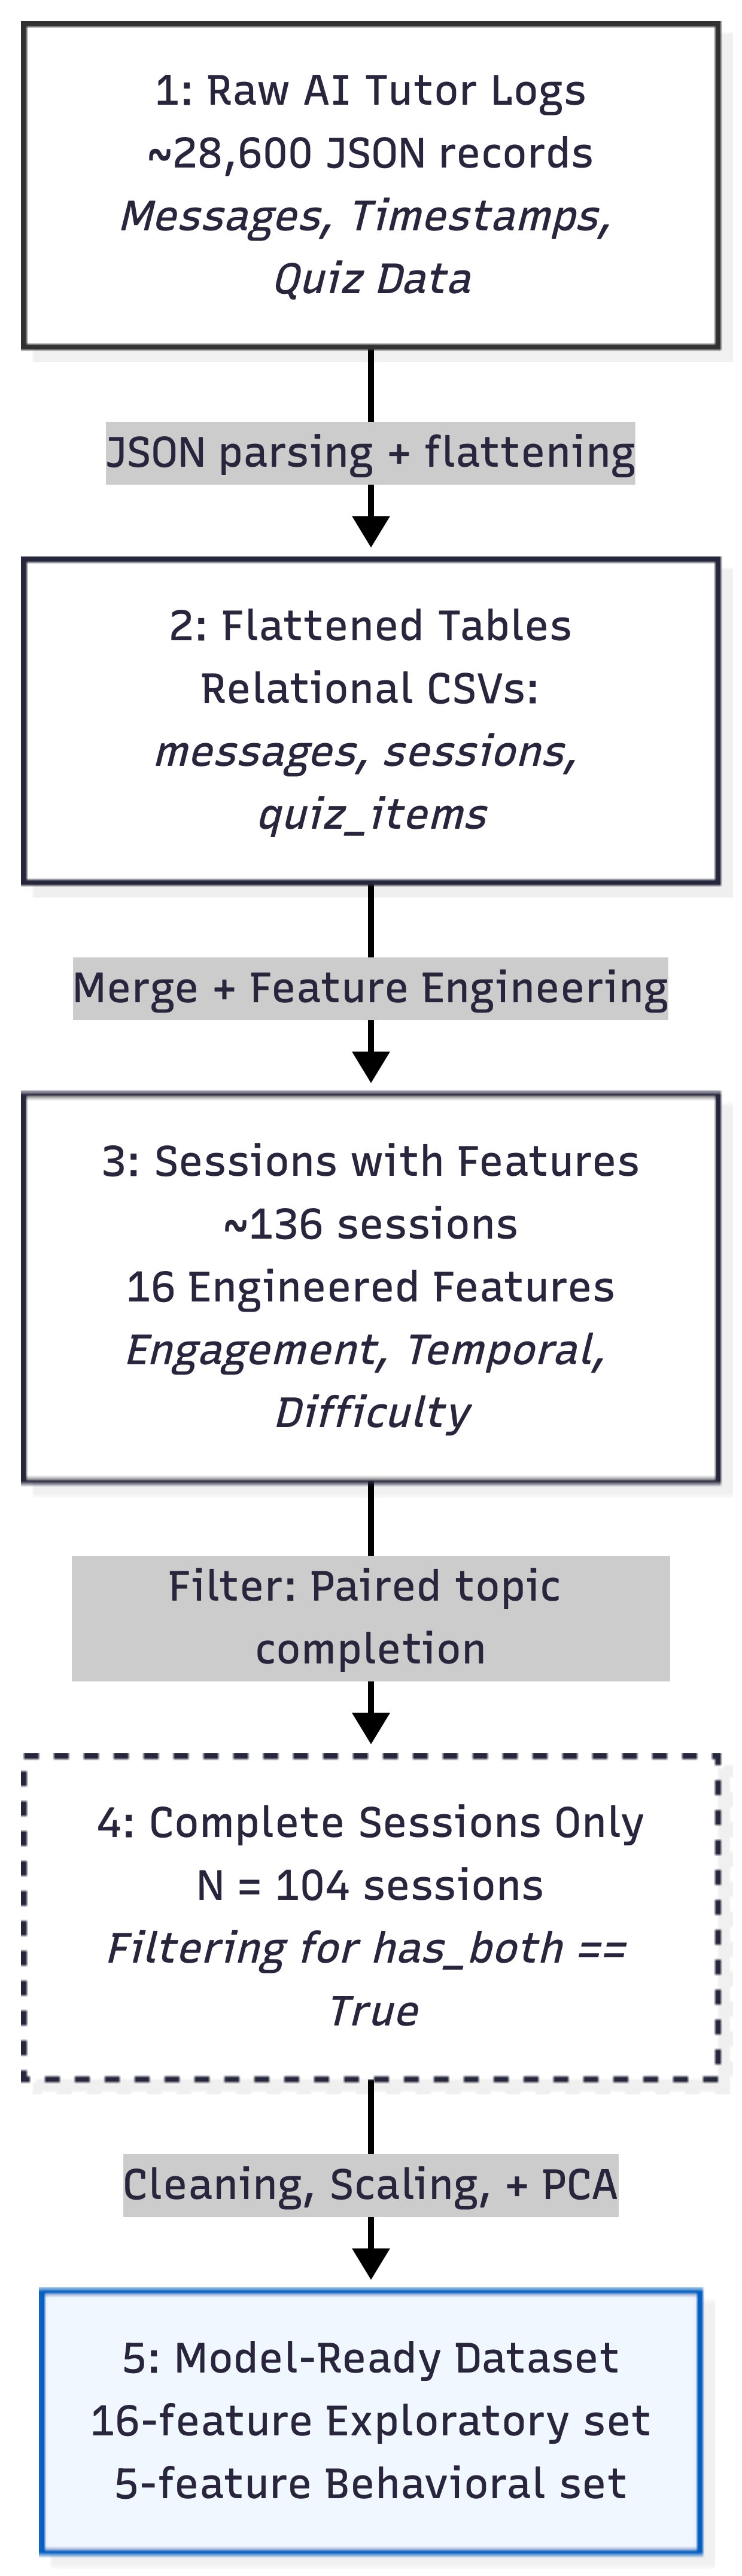
\includegraphics[width=.75\linewidth, height=0.35\textheight, keepaspectratio]{AI Tutor Log Processing-2026-04-23-232835.png}

    \caption{Preprocessing Pipeline}
    \label{fig:placeholder}
\end{figure}

\subsection{JSON Parsing and Flattening}
The first stage involved converting the nested JSON logs into relational tables. Three primary tables were produced:

\begin{itemize}[noitemsep]
    \item \textbf{messages.csv}: one row per message, containing sender (user or assistant), timestamp, and message text.
    \item \textbf{sessions.csv}: one row per session, containing session-level metadata such as topic, instructional condition, and duration.
    \item \textbf{quiz.csv}: one row per quiz item, including correctness and difficulty level.
\end{itemize}

Flattening the logs enabled feature engineering at both the message level (e.g., response times) and the session level (e.g., total messages, duration).

\subsection{Session Merging and Feature Assembly}
The flattened tables were merged into a unified dataset, \texttt{sessions\_with\_engagement\_features.csv}, which contained all engineered features required for modeling. This merge included:

\begin{itemize}[noitemsep]
    \item computing response-time features by differencing consecutive message timestamps,
    \item aggregating message counts (total, user, assistant),
    \item calculating rapid-response indicators,
    \item attaching quiz-level difficulty information,
    \item computing session duration from the first to last timestamp.
\end{itemize}

This produced the full 16-feature set used in the exploratory analysis.

\subsection{Filtering for Complete Sessions}
A critical preprocessing step was filtering to sessions where students completed \emph{both} topics (ArrayList and Recursion). This was implemented using the boolean field \texttt{has\_both}.

This filter reduced the dataset from approximately 136 sessions to 104 complete sessions, ensuring that every record had a valid quiz score and preventing target-missingness issues. Restricting to repeated sessions also reduced topic-specific bias.

\subsection{Cleaning and Imputation}
Several fields required cleaning:

\begin{itemize}[noitemsep]
    \item missing difficulty values were imputed with 0,
    \item response-time nulls were filled with the median response time for that session,
    \item boolean fields were converted to integers,
    \item categorical fields (e.g., session type, instructional condition) were label-encoded.
\end{itemize}

These steps ensured that all features were numeric and compatible with downstream models.

\subsection{Scaling}
All numeric features were standardized using \texttt{StandardScaler}, producing zero-mean, unit-variance inputs. Scaling was particularly important for SVM and PCA, which are sensitive to feature magnitude.

\subsection{Dimensionality Reduction (PCA)}
Principal Component Analysis (PCA) was applied to the full 16-feature set to examine structure in the data and support linear models. PCA revealed that 7--8 components captured approximately 90\% of variance. PC1 loaded heavily on response-time variability and pacing, while PC2 captured session duration and difficulty-weighted correctness.

\begin{figure}
    \centering
    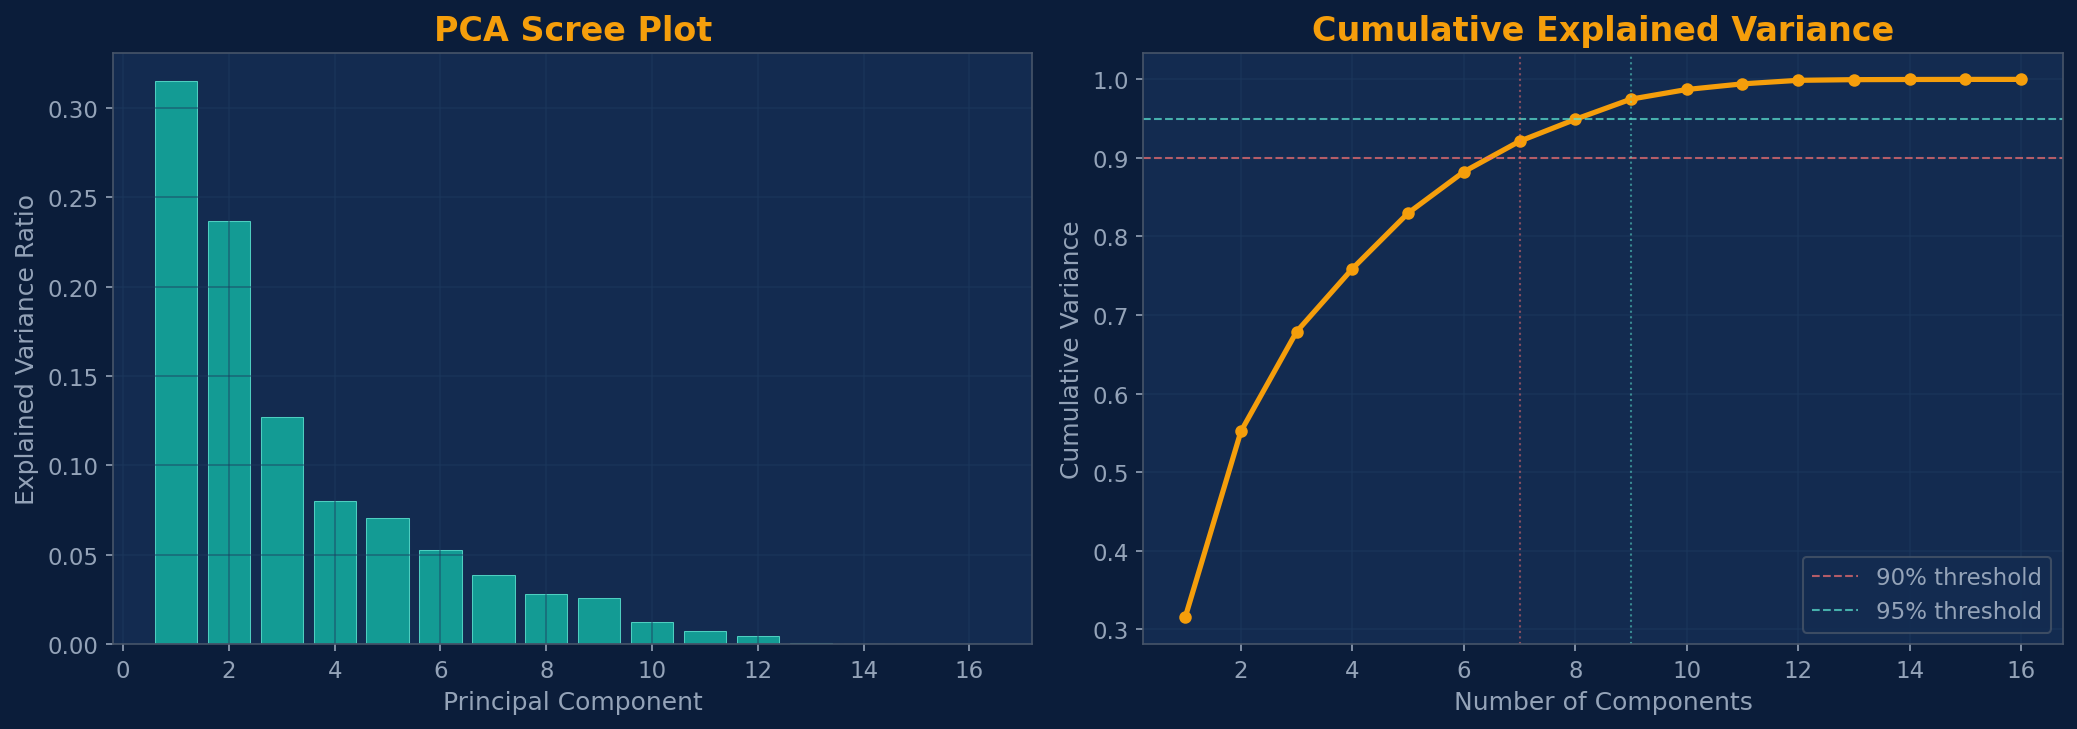
\includegraphics[width=1\linewidth]{pca_scree.png}
    \caption{Variance explained by PCA components.}
    \label{fig:placeholder}
\end{figure}

\subsection{Leakage Identification and Feature Refinement}
During feature importance analysis, we identified a critical issue with the difficulty-weighted features (Fig \ref{fig:importance}): avg\_difficulty\_correct and avg\_difficulty\_incorrect). These features are derived directly from quiz question answer, meaning they partially encode the target variable (quiz score). Including quiz-adjacent features to predict quiz scores affects model performance and misrepresents genuine behavioral prediction.

\begin{figure}
    \centering
    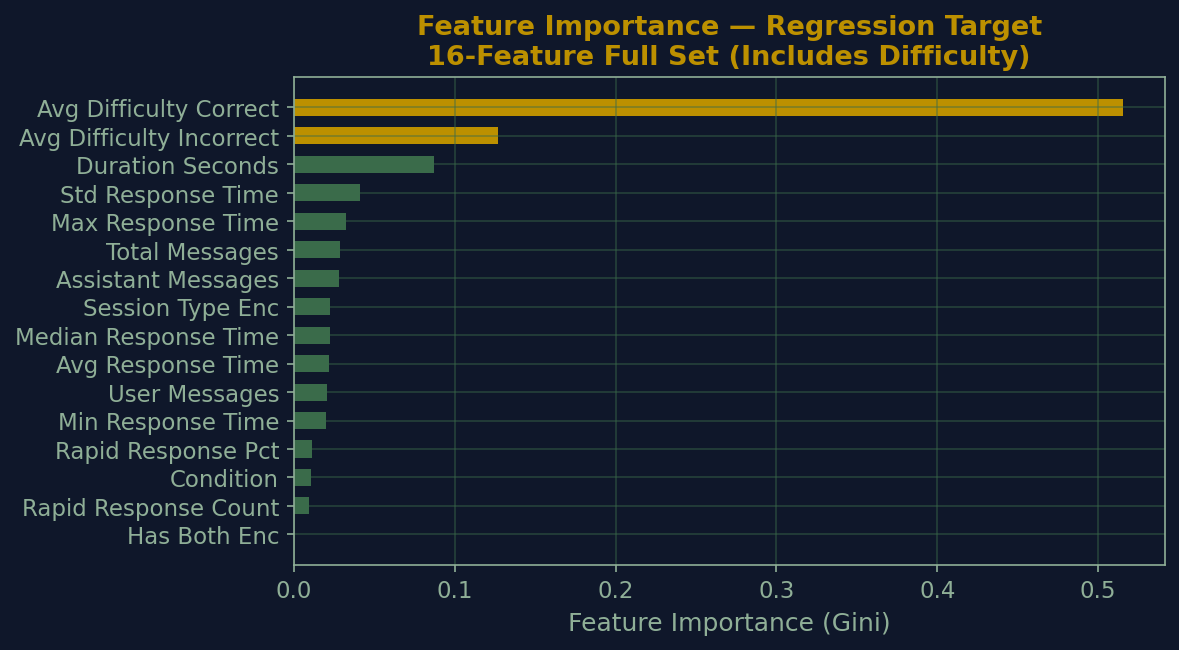
\includegraphics[width=1\linewidth]{16feat_full_feature_importance.png}
    \caption{Feature Importance Reveals Leaked Features Highly Influential}
    \label{fig:importance}
\end{figure}

Additionally, the five response-time variants (avg, median, std, min, max) capture highly correlated information, with avg\_response\_time providing the strongest and most interpretable signal. min\_response\_time was the original pacing feature, and reflects a single moment rather than sustained behavioral patterns. It was replaced later by average\_response\_time in the final pipeline.

To address the leakage issues, we refined the dataset to a five-feature behavioral-only model containing no quiz-derived information: 

\begin{itemize}[noitemsep]
    \item condition,
    \item session\_type\_enc,
    \item duration\_seconds,
    \item total\_messages,
    \item avg\_response\_time.
\end{itemize}

Results from this model represent the more rigorous and scientifically defensible claim: that session behavior alone, without any quiz performance data, can predict learning outcomes above chance.


This final dataset was used for the primary scientific analysis and represents the most defensible modeling claim.


\section{Machine Learning Models}
We evaluate Logistic Regression, Random Forest, Gradient Boosting, and SVM (RBF). All models use an 80/20 stratified split and 5-fold cross-validation.

\section{Results}

\subsection{ Model Performance on the Full 16‑Feature Set}
Table \ref{fig:importance} summarizes performance across all four classifiers using the full engineered feature set, which includes difficulty‑weighted correctness features. These results represent the maximum extractable signal from the dataset, but—as shown later—are inflated by data leakage.

Across models, test accuracy ranged from 0.57 to 0.67, with Gradient Boosting achieving the strongest AUC‑ROC (0.791) and perfect training accuracy (1.00). This large train–test gap indicates overfitting, driven by the model’s reliance on difficulty‑weighted features that partially encode quiz correctness. Random Forest shows a similar pattern, with high training accuracy (0.952) and lower cross‑validated performance (0.577 ± 0.102).

SVM (RBF) demonstrates the most stable generalization (0.681 CV accuracy), suggesting that kernel‑based models capture genuine behavioral structure even when noisy or leaky features are present.
These results motivated the refinement to a leakage‑free behavioral feature set.

\subsection{ Model Performance on the Refined 5‑Feature Behavioral Set}

After removing difficulty‑weighted features, model performance reflects purely behavioral prediction. Table 2 shows that Gradient Boosting achieves the strongest overall performance on the clean feature set:
\begin{itemize}
    \item 0.78 test accuracy
    \item 0.72 cross‑validated accuracy
    \item 0.87 AUC‑ROC
\end{itemize}


This indicates that even without correctness‑adjacent features, behavioral traces alone contain meaningful predictive signal.
SVM (RBF) also performs competitively (0.70 CV accuracy), confirming that nonlinear boundaries are appropriate for this dataset. Logistic Regression performs surprisingly well (0.70 test accuracy), suggesting that even a linear decision boundary captures important behavioral structure.

Random Forest improves substantially on the behavioral‑only set (0.70 CV accuracy), indicating that removing leakage stabilizes tree‑based models.
\subsection{ Confusion Matrix Analysis}
Confusion matrices reveal distinct model behaviors:
Gradient Boosting achieves the highest recall for high performers, correctly identifying 9 of 10 students scoring $\geq 70\%$
This makes it the strongest candidate for early‑intervention systems where missing a struggling student is costly.
SVM (RBF) provides the most balanced classification, with strong performance on both classes and fewer extreme errors.
Logistic Regression and Random Forest show moderate, stable performance, correctly identifying 7 high performers each.
Across all models, misclassifications cluster in the 60–75\% quiz range, indicating that borderline students exhibit ambiguous behavioral patterns that are inherently harder to classify.
This “borderline error zone” is consistent with educational data mining literature: students near mastery thresholds often show mixed behavioral signals.
\subsection{ Feature Importance and SHAP Interpretability}

Interpretability analyses were conducted using both model‑based (Random Forest Gini importance) and model‑agnostic (SHAP) methods.
On the full 16‑feature set, difficulty‑weighted features dominate importance rankings, confirming leakage. However, timing and pacing features still contribute meaningfully.

On the refined 5‑feature behavioral model, SHAP reveals a consistent global pattern:
\begin{itemize}
    \item duration\_seconds is the strongest predictor
    \item session\_type\_enc and condition provide structural context
    \item avg\_response\_time captures pacing and cognitive load
    \item total\_messages reflects engagement depth
\end{itemize}

The agreement between Gini importance and SHAP strengthens confidence that these behavioral signals are robust and not artifacts of a single model.

 \subsection{Ablation Study}
 

Logistic Regression and SVM improve when difficulty features are removed (+0.03 to +0.10), suggesting that these features introduce noise for models that rely on smooth decision boundaries.
Random Forest shows moderate sensitivity, improving stability on the behavioral‑only set.

This asymmetry provides direct evidence that difficulty‑weighted features artificially inflate performance for tree‑based models, while behavioral‑only features produce cleaner, more generalizable predictions.

\begin{table}
\centering
\caption{Model Performance Results}
\begin{tabular}{|p{2cm}|p{1cm}|p{1cm}|p{1cm}|p{1cm}|p{1.6cm}|}
\hline
\textbf{Model} & \textbf{Train} & \textbf{Test} & \textbf{F1} & \textbf{AUC} & \textbf{ACC 5-fold}\\
\hline
Logistic Regression  & 0.675 & 0.571  & 0.566  & 0.591 & 0.591 \\
\hline
Random Forest & 0.952 & 0.667  & 0.667 & 0.673 &  0.577±0.102 \\
\hline
Gradient Boosting & 1.000 & 0.667  & 0.667 & 0.791 &  0.624±0.126 \\
\hline
SVM (RBF) & 0.735 & 0.571  & 0.566 & 0.618 &  0.681±0.094 \\
\hline
\end{tabular}
\label{tab:performance-chart}
\end{table}

\subsection{Refined 5-Feature Behavioral Model}
SVM (RBF) achieves: NEED TO REPLACE WITH GRADIENT BOOSTING
\begin{itemize}[noitemsep]
    \item 71.4\% test accuracy
    \item 68.1\% CV accuracy
    \item 0.764 AUC-ROC
\end{itemize}

\begin{figure}[t]
    \centering
    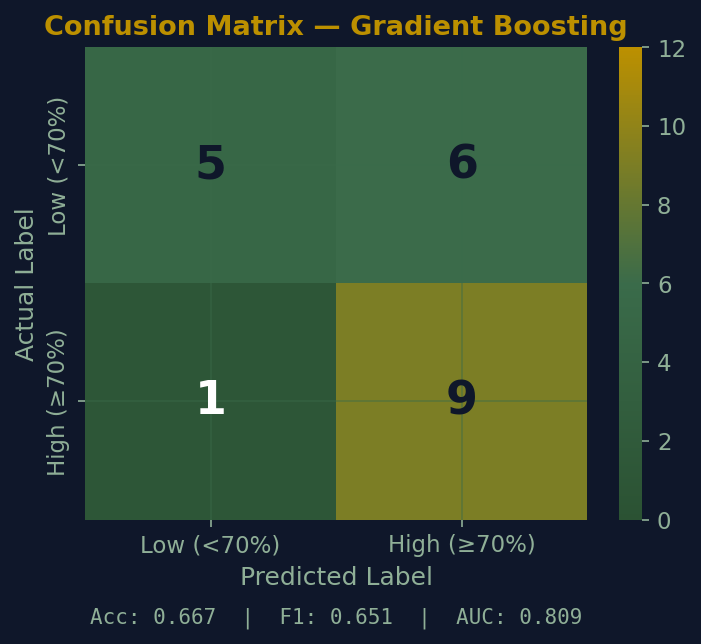
\includegraphics[width=0.45\textwidth]{5feat_behavioral_confusion_Gradient_Boosting.png}
    \caption{Confusion matrix for Gradient Boosting.}
    \label{fig:gb_confusion}
\end{figure}


\subsection{SHAP Interpretability}
% FIGURE PLACEHOLDER
\begin{figure}[t]
    \centering
    \fbox{\begin{minipage}{0.75\linewidth}
    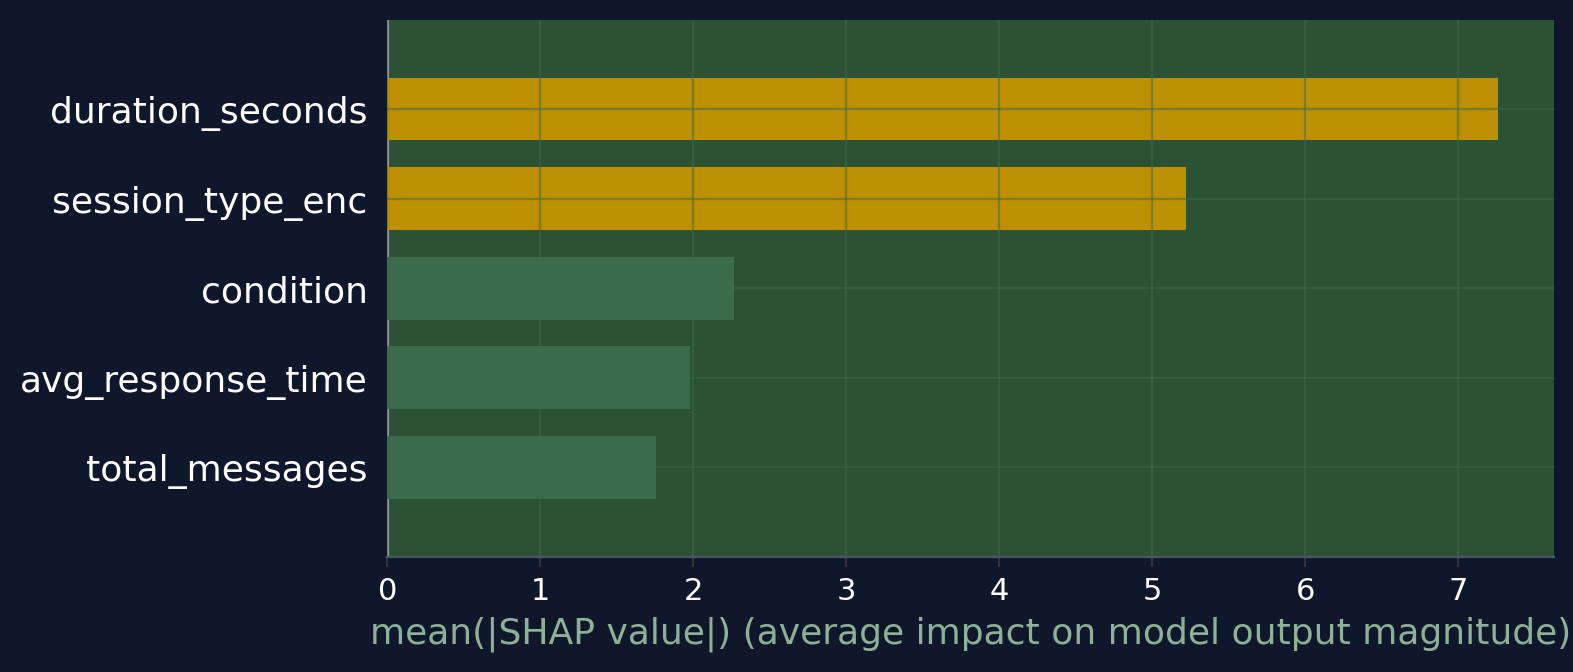
\includegraphics[width=.90\linewidth, height=0.90\textheight, keepaspectratio]{shap_bar_5feat_behavioral.png}
    \end{minipage}}
    \caption{SHAP feature importance for the 5-feature model.}
\end{figure}

\subsection{Ablation Study}
% TABLE PLACEHOLDER
\begin{table}[t]
\centering
\caption{TODO: Ablation Study Results}
\begin{tabular}{lll}
\toprule
Model & CV Before & CV After \\
\midrule
GBM & -0.14 & -0.29 \\
SVM & +0.04 & +0.08 \\
\bottomrule
\end{tabular}
\end{table}


\section{Related Work}


Research in Artificial Intelligence in Education (AIED) spans intelligent tutoring systems, adaptive feedback, and student modeling \cite{woolf2013aied}. Early intelligent tutoring systems (ITS) relied on rule‑based and model‑tracing architectures to provide structured scaffolding and individualized support, demonstrating consistent learning gains in domains such as programming \cite{koedinger2015learning, koedinger2015cognitive}. Machine learning has long played a role in these systems: tutors use ML techniques to infer student knowledge, identify learning strategies, and adapt instruction based on patterns in tutor–student interactions \cite{woolf2013aied, saeed2022mlreview}. These approaches show that behavioral traces, rather than correctness alone, can serve as meaningful signals for personalization.

Educational Data Mining (EDM) has further established that behavioral features such as timing, pacing, hesitation, and engagement depth carry predictive value for student performance \cite{romero2010edm, baker2009state}. Large‑scale studies of internet usage and LMS clickstream data demonstrate that interaction behaviors can differentiate performance groups and support early identification of at‑risk learners \cite{xu2019internetusage, borna2024}. Recent MOOC research similarly shows that event‑level interaction logs can be used to cluster learners and predict behavioral trajectories with high accuracy \cite{chonraksuk2024thaiMOOC}. However, these studies primarily rely on platform‑level telemetry rather than the fine‑grained, session‑level conversational interactions produced by AI tutors.

Clickstream‑based predictive modeling has been applied to early warning systems, but accurately predicting high achievers remains challenging, highlighting the need for more nuanced behavioral models \cite{borna2024, tang2025multiverse}. Within programming education, prior work has focused on IDE telemetry, code snapshots, and compilation events as predictors of learning outcomes \cite{piech2015deep, rivers2017automated}. These signals capture problem‑solving behavior but do not reflect the conversational dynamics of LLM‑mediated tutoring.

Recent work has begun evaluating LLM‑based tutoring for learning gains and user experience \cite{kasneci2023chatgpt}, and explainable ML studies illustrate how interpretable models (e.g., SHAP with tree models) can surface influential predictors in educational settings \cite{info16090763}. Yet, relatively little research treats conversational interaction logs themselves as a behavioral dataset for predictive modeling.

This study builds on these strands by showing that session‑level behavioral features extracted from LLM tutor interactions can predict short‑term quiz performance even when correctness‑based features are excluded. We also identify a methodological risk—difficulty‑weighted quiz features can leak target information—and demonstrate that removing such features yields more defensible, generalizable models.


\section{Uniqueness}

Many predictive models in education rely on demographic variables, prior academic history, or socio‑economic indicators. While these features often improve accuracy, they risk reinforcing existing inequities by embedding structural biases into algorithmic predictions. Behavioral‑only models offer a more equitable alternative: they rely solely on how a student interacts with the learning environment, not who the student is or what background they come from. By focusing on pacing, duration, and message patterns, this study avoids demographic proxies and instead models the learning process itself. The ablation study confirms that these behavioral features are sufficient to predict performance above chance, even when correctness‑adjacent features are removed. This approach aligns with emerging ethical guidelines in AIED, emphasizing fairness, transparency, and the minimization of bias in algorithmic decision‑making.

\section{Discussion}


A major challenge in current Educational Data Mining (EDM) is that predictive models are often built on historical, post-hoc data such as final grades or weekly LMS activity. These approaches limit the ability to intervene during learning and risk perpetuating socio-economic or demographic biases. In contrast, this study reframes the problem by treating a live, chat-based generative AI tutoring session as a supervised machine learning task using real-time interaction logs.

The ablation study demonstrates that pure behavioral traces—pacing, duration, and message volume—predict learning outcomes independently of quiz-derived features. This strictly behavioral approach mitigates demographic bias and is highly actionable: if an AI tutor detects erratic pacing or rapid, shallow responses, the system can dynamically adjust scaffolding depth or trigger metacognitive prompts before the assessment phase.

This work also addresses the ``black box'' criticism frequently directed at AI systems in education. By applying explainable AI (XAI) techniques, specifically SHAP, we show that session duration and message volume are the primary drivers of model predictions. This transparency enables educators to understand the behavioral factors contributing to a student's struggle, fostering trust in the AI's diagnostic capabilities.

A persistent limitation of traditional educational analytics is their reliance on post‑hoc data such as final grades, weekly LMS activity, or end‑of‑unit assessments. These retrospective signals arrive too late to support students during the learning process, limiting their usefulness for timely intervention. Real‑time prediction, by contrast, enables formative assessment: identifying struggling students while they are still engaged in the learning activity. In AI tutoring environments, this capability is especially powerful. If the system detects erratic pacing, rapid guessing, or shallow engagement, it can immediately adjust the level of scaffolding, slow down the instructional sequence, or trigger metacognitive prompts. This transforms the AI tutor from a passive content delivery tool into an adaptive, diagnostic system capable of supporting students before misconceptions solidify. The present study demonstrates that such real‑time behavioral prediction is feasible using only interaction logs.

Additionally, Many predictive models in education rely on demographic variables, prior academic history, or socio‑economic indicators. While these features often improve accuracy, they risk reinforcing existing inequities by embedding structural biases into algorithmic predictions. Behavioral‑only models offer a more equitable alternative: they rely solely on how a student interacts with the learning environment, not who the student is or what background they come from. By focusing on pacing, duration, and message patterns, this study avoids demographic proxies and instead models the learning process itself. The ablation study confirms that these behavioral features are sufficient to predict performance above chance, even when correctness‑adjacent features are removed. This approach aligns with emerging ethical guidelines in AIED, emphasizing fairness, transparency, and the minimization of bias in algorithmic decision‑making.

Finally, the findings offer a practical solution to the human–AI tradeoff currently debated in educational policy. Rather than replacing human educators, the AI tutor functions as a sensitive diagnostic engine. When the model detects behavioral patterns strongly correlated with failure, it can flag the student for human intervention, allowing instructors to provide the relational empathy and nuanced support that algorithms cannot replicate.

\section{Conclusion}

\subsection {The Impact of Feature Refinement and Leakage Removal}

Initial modeling on the full 16-feature set yielded performance metrics that, while seemingly strong, were identified as being artificially inflated by data leakage. Feature importance analysis revealed that difficulty-weighted metrics—derived from quiz responses—partially encoded the target variable. This realization necessitated a pivot to a more rigorous analytical narrative focused exclusively on session-level behavioral signals.


\subsection{Performance Gains from Behavioral Features}

Contrary to the expectation that reducing the feature count would diminish predictive power, the transition to a five-feature behavioral model resulted in a cleaner signal and improved generalization. While the initial models exhibited significant train-test gaps indicative of overfitting, the refined behavioral set stabilized the learning process.


On this optimized dataset, Gradient Boosting emerged as the superior classifier, achieving a test accuracy of 0.78 and an AUC-ROC of 0.87. Other models also demonstrated marked improvements; SVM (RBF) achieved a stable cross-validated accuracy of 68.1%, while Logistic Regression and Random Forest benefited from the removal of noisy, quiz-adjacent features. These findings indicate that the "how" of student interaction—characterized by pacing and duration—is more predictive of short-term learning outcomes than the specific difficulty of content mastered during the session.


\subsection{Interpretability and Behavioral Signals}

The convergence of SHAP values and Gini importance confirms that session duration, message pacing (average response time), and engagement depth (total messages) are the most robust indicators of academic mastery. The fact that these bare-bones traces can predict success with high confidence (0.87 AUC) suggests that AI tutoring systems can identify at-risk students in real-time based solely on conversational cadence.


\subsection{Practical Implications for Adaptive Learning}

This study demonstrates that interaction-log features provide a non-intrusive, real-time mechanism for diagnostic assessment. By prioritizing behavioral signals over performance-based metrics, tutoring systems can mitigate the risks of data leakage and provide pedagogical interventions—such as adjusting scaffolding depth or triggering metacognitive prompts—well before a student reaches the final assessment phase. These results position the AI tutor not as a static instructional tool, but as a sensitive diagnostic engine capable of flagging behavioral patterns associated with cognitive struggle
\bibliographystyle{IEEEtran}
\bibliography{references}

\end{document}
